\documentclass[11pt,a4paper]{article}
\usepackage[utf8]{inputenc}
\usepackage[T1]{fontenc}
\usepackage[margin=2.4cm]{geometry}
\usepackage{graphicx}
\usepackage{booktabs}
\usepackage{float}
\usepackage{hyperref}
\setlength{\parindent}{0pt}
\setlength{\parskip}{0.7em}

\begin{document}

\pagenumbering{gobble}
\begin{titlepage}
\centering
\vspace*{1.5cm}

{\Large Evaluation, Deployment and Monitoring of Models\par}
\vspace{1.4cm}

{\large Task: XAI3\par}
\vspace{0.4cm}

{\LARGE\bfseries Model-Agnostic Methods: Partial Dependence Plots\par}
\vspace{1.8cm}

{\large\bfseries Authors\par}
\vspace{0.2cm}
Jose Miguel García Ríos\par
Daniel Herrán Gómez-Senent\par
Batu Senyucel\par
\vspace{1.4cm}

{\large\bfseries Subject\par}
\vspace{0.2cm}
Evaluation, Deployment and Monitoring of Models\par
\vspace{1.4cm}

{\large\bfseries Date\par}
\vspace{0.2cm}
May 4, 2026\par

\vfill
\end{titlepage}

\clearpage
\pagenumbering{roman}
\tableofcontents
\newpage

\clearpage
\pagenumbering{arabic}

\section{Introduction}

This report solves Exercise 5 on model-agnostic Partial Dependence Plots (PDP).
The objective is to fit random forest regression models and use PDPs to interpret
how selected input variables affect the predicted target.

For the bike rental problem, the target variable is \texttt{cnt}. The daily bike
dataset was used because the question asks for the influence of days since 2011.
The model uses calendar, weather, and day-type variables, including
\texttt{days\_since\_2011}, \texttt{temp}, \texttt{hum}, and \texttt{windspeed}.

For the house price problem, the target variable is \texttt{price}. The model uses
\texttt{bedrooms}, \texttt{bathrooms}, \texttt{sqft\_living}, \texttt{sqft\_lot},
\texttt{floors}, and \texttt{yr\_built}, as requested in the exercise.

All random choices use a fixed seed of 42. The PDPs are generated with
\texttt{scikit-learn}. Random samples are used for the larger house dataset and
for the bidimensional PDP step, following the warning in the exercise statement.

\section{Data Preparation and Models}

The bike-sharing data contain daily rental counts and weather/calendar variables.
The original date field is transformed into \texttt{days\_since\_2011}, which is
the variable requested in the statement. The target is the total number of daily
rentals, \texttt{cnt}. The variables \texttt{casual} and \texttt{registered} are
excluded because they sum directly to \texttt{cnt} and would leak the answer.

The house-price data are modelled with the variables requested in the task:
\texttt{bedrooms}, \texttt{bathrooms}, \texttt{sqft\_living}, \texttt{sqft\_lot},
\texttt{floors}, and \texttt{yr\_built}. The target is \texttt{price}. Random
forest regressors are used in both exercises because they provide flexible
non-linear approximations while remaining compatible with model-agnostic PDP
analysis.

\begin{table}[H]
\centering
\begin{tabular}{lrr}
\toprule
Model & Test $R^2$ & Test MAE \\
\midrule
Bike rentals & 0.873 & 450.43 rentals \\
House prices & 0.610 & 156,514.67 USD \\
\bottomrule
\end{tabular}
\caption{Validation metrics for the random forest regressors.}
\end{table}

\section{One-Dimensional PDP for Bike Rentals}

\begin{figure}[H]
\centering
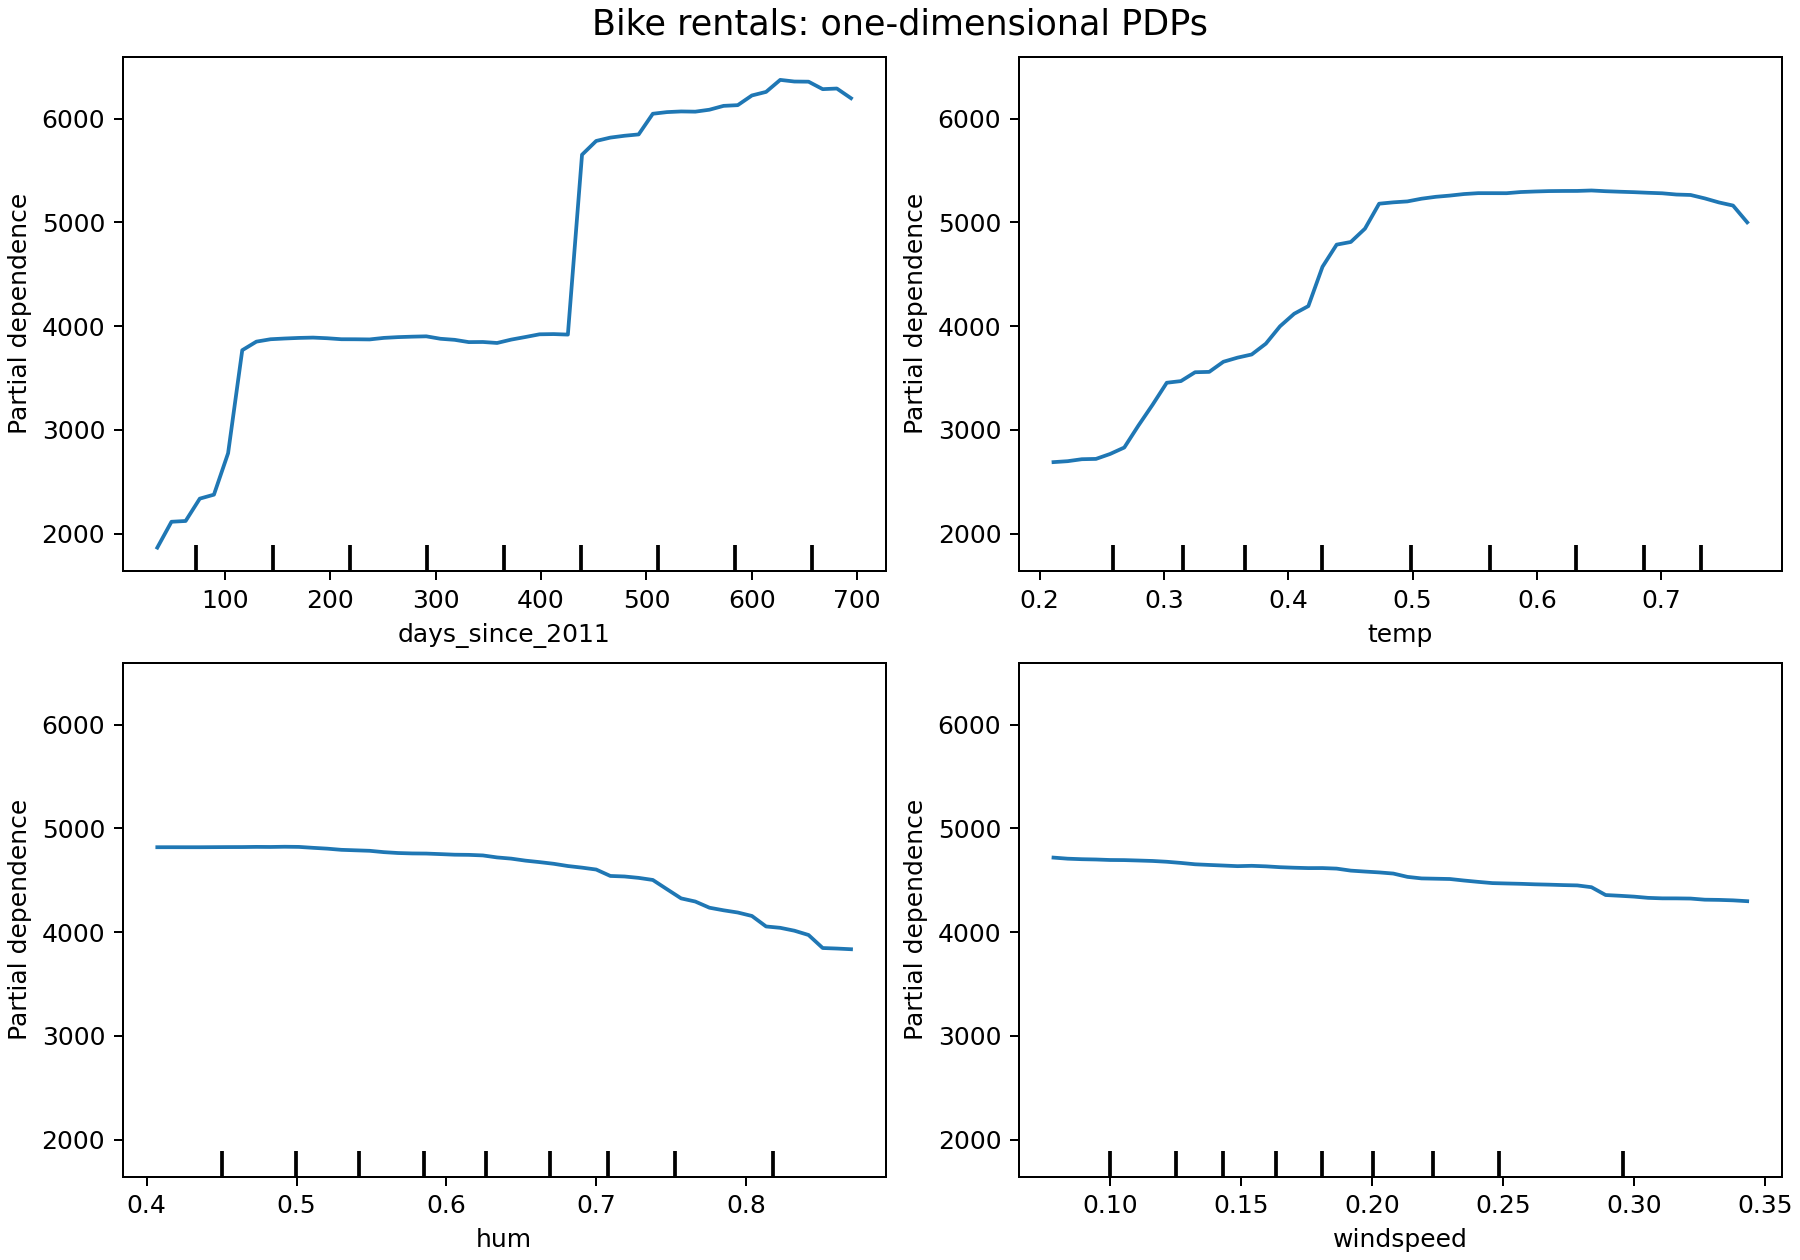
\includegraphics[width=\textwidth]{figures/bike_1d_pdp.png}
\caption{One-dimensional PDPs for days since 2011, temperature, humidity, and wind speed.}
\end{figure}

\textbf{Influence of days since 2011.} The PDP shows a clear increasing tendency:
predicted bike rentals are lower at the beginning of the period and higher later.
This suggests that the model learned a temporal growth effect, probably combining
real demand growth with yearly and seasonal patterns present in the data.

\textbf{Influence of temperature.} Temperature has a strong positive effect.
Predicted bike counts rise as temperature increases from cold to moderate/warm
values. The increase becomes weaker at the highest temperatures, so the model does
not treat heat as unlimitedly beneficial.

\textbf{Influence of humidity.} Humidity has a negative effect. The model predicts
more rentals at low or medium humidity and fewer rentals when humidity becomes
high. This is reasonable because humid weather is usually less comfortable for
cycling.

\textbf{Influence of wind speed.} Wind speed is mostly negative at higher values.
The effect is weaker and noisier than temperature or humidity, but the model still
learns that stronger wind tends to reduce expected rentals.

\section{Bidimensional PDP for Humidity and Temperature}

\begin{figure}[H]
\centering
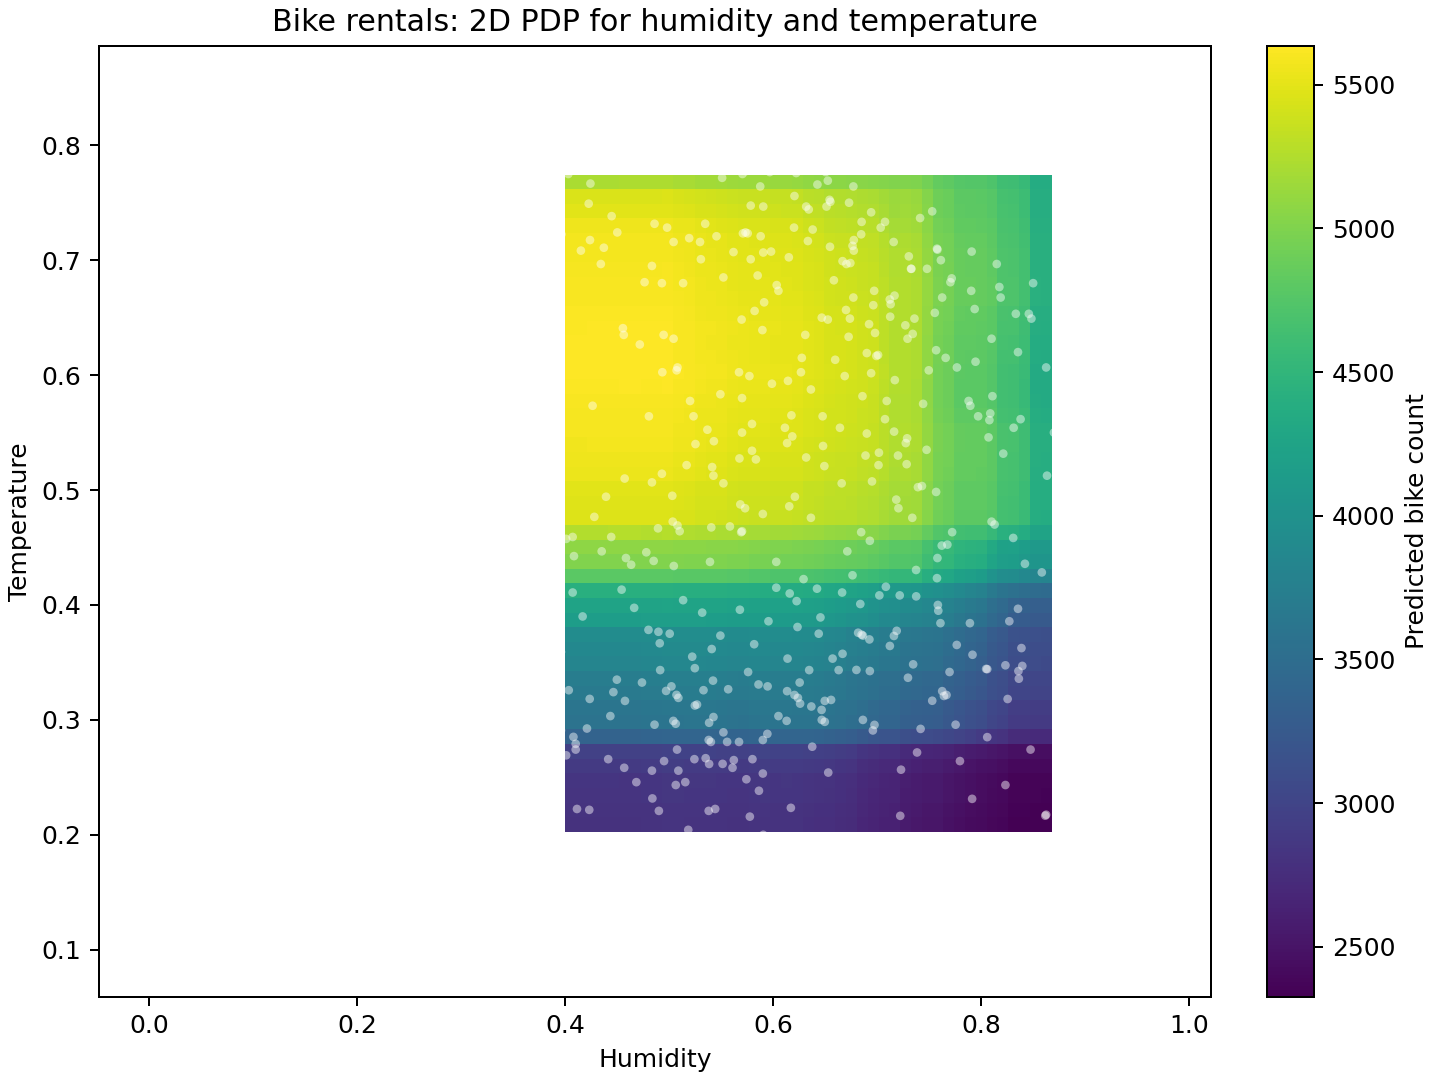
\includegraphics[width=0.82\textwidth]{figures/bike_2d_pdp_hum_temp.png}
\caption{Bidimensional PDP for humidity and temperature. White points show the sampled input distribution.}
\end{figure}

The 2D PDP confirms that temperature and humidity interact in the bike rental
model. The highest predicted rental counts appear in warm conditions with low to
medium humidity. The lowest predictions appear in cold conditions and also in
areas with high humidity. Temperature is the dominant positive driver, but high
humidity reduces the expected demand even when temperature is favorable.

The point overlay shows where observed combinations of humidity and temperature
are concentrated. This is important because PDP regions with very few observed
points should be interpreted cautiously: they represent model extrapolation more
than strongly supported data behavior.

\section{PDP for House Price}

\begin{figure}[H]
\centering
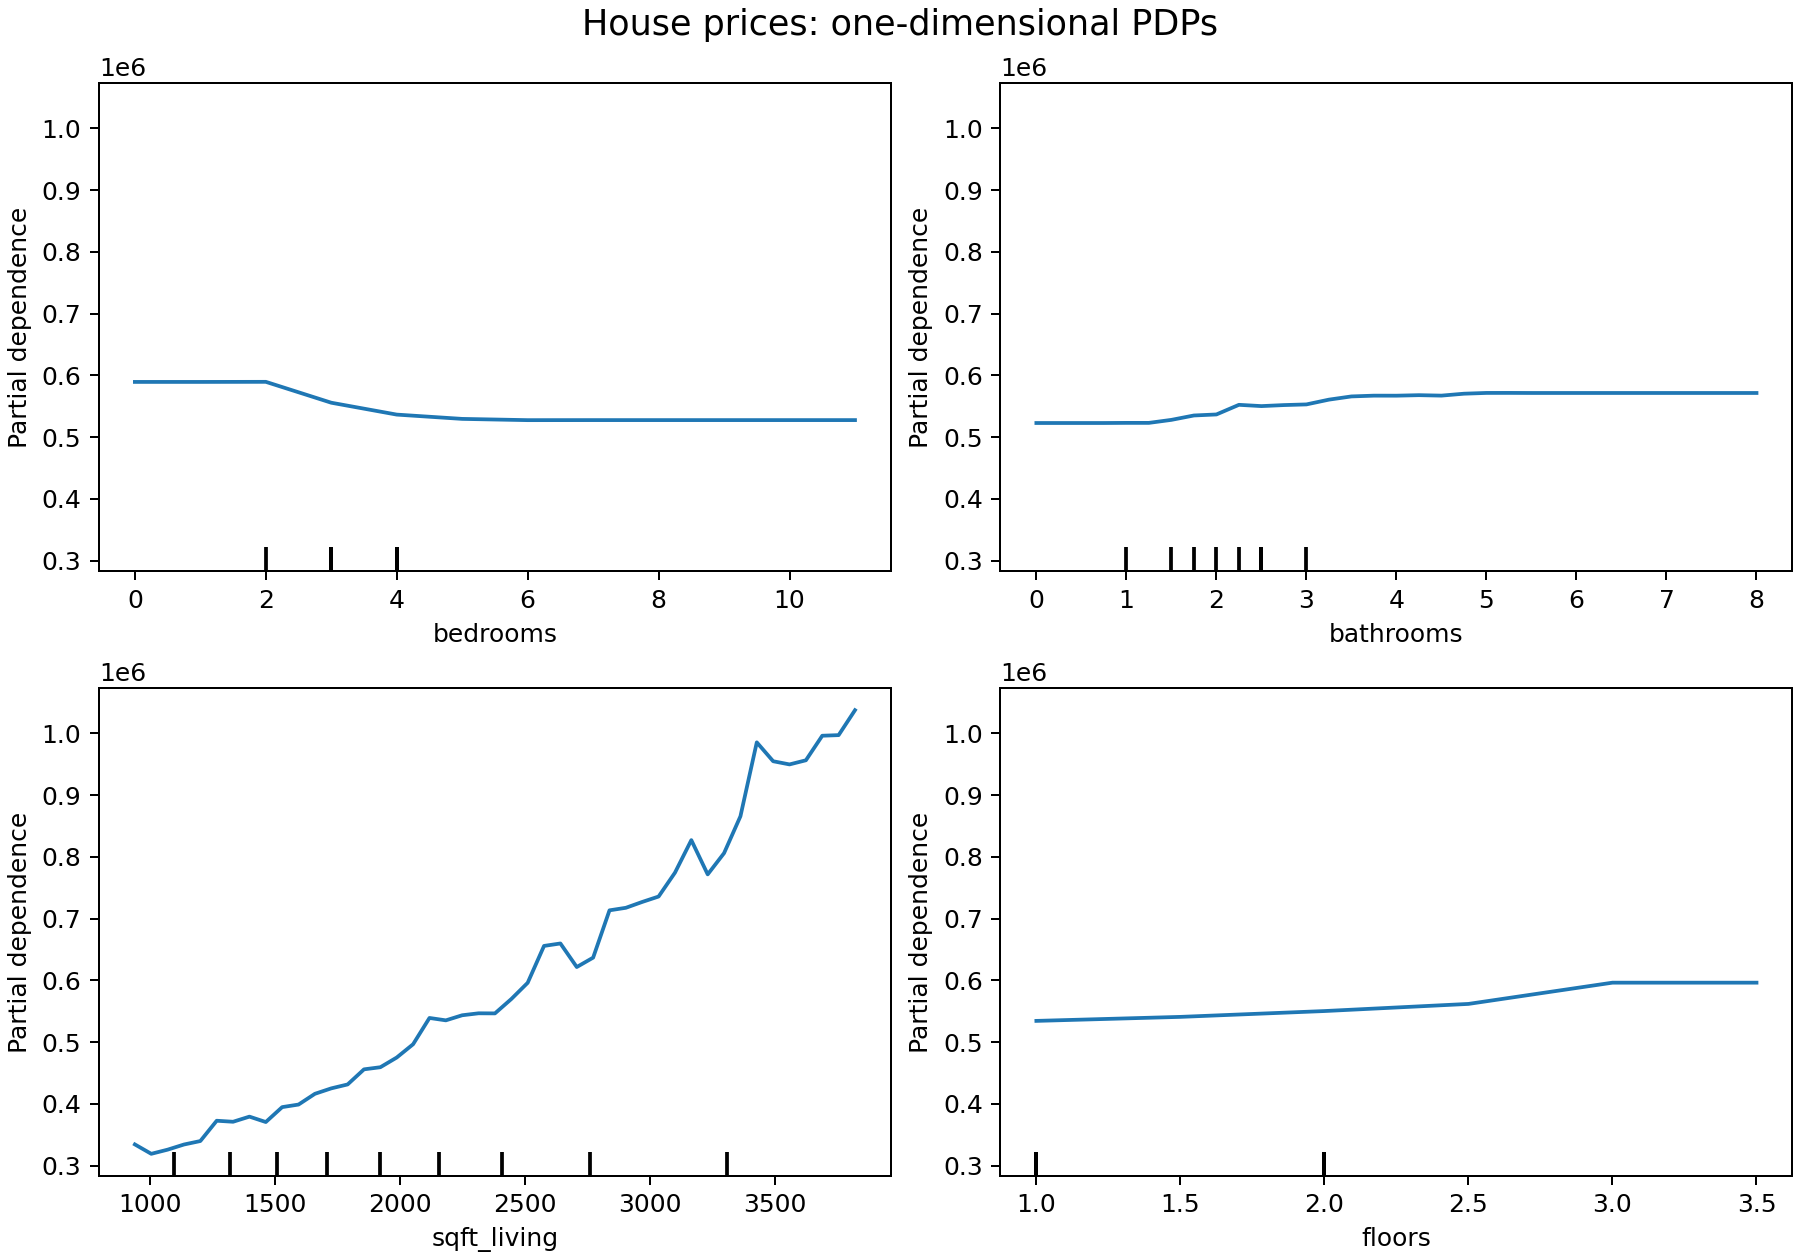
\includegraphics[width=\textwidth]{figures/house_1d_pdp.png}
\caption{One-dimensional PDPs for bedrooms, bathrooms, living area, and floors.}
\end{figure}

\textbf{Influence of bedrooms.} Bedrooms do not have a simple strong positive
relationship with price. The PDP is comparatively flat and slightly irregular,
which means bedroom count alone is not the main driver once bathrooms, living
area, lot size, floors, and year built are also included. Very high bedroom
counts should be interpreted carefully because they are uncommon.

\textbf{Influence of bathrooms.} Bathrooms have a positive effect. Houses with
more bathrooms are predicted to be more expensive, especially when moving from
small values to medium/high values. This likely captures both comfort and the fact
that larger houses often include more bathrooms.

\textbf{Influence of sqft\_living.} Living area is the strongest and clearest
predictor among the requested variables. The PDP rises as \texttt{sqft\_living}
increases, meaning the random forest predicts higher prices for larger houses.
The increase is steep over common living-area values and then becomes less stable
at the largest values, where there are fewer observations.

\textbf{Influence of floors.} Floors have a weaker effect than living area and
bathrooms. The model gives somewhat higher predictions for houses with more
floors, but the relationship is not as strong or as smooth. This suggests that
floor count is useful mainly together with other structural variables.

\section{Practical Implications and Limitations}

The PDPs are useful because they turn a random forest into readable marginal
effects. For bike rentals, the plots can support operational planning: more bikes
and rebalancing effort are expected to be needed on warm, relatively dry days and
in the later period of the service. For house prices, the PDPs show that living
area and bathrooms are stronger price drivers than bedroom count alone.

There are also limitations. PDPs average over the full data distribution, so they
can hide individual-level differences and interactions. The two-dimensional PDP
partly solves this for humidity and temperature, but regions with few observed
points should still be interpreted carefully. Finally, these models are
predictive and explanatory, not causal: the plots show what the fitted random
forest learned, not guaranteed causal effects in the real world.

\section{Conclusion}

The PDP analysis gives interpretable summaries of the random forest models. For
bike rentals, time and temperature increase predicted demand, while humidity and
wind speed reduce it. The 2D PDP shows that warm and relatively dry weather gives
the highest predicted rental counts. For house prices, living area is the dominant
positive factor, bathrooms also increase predicted prices, while bedrooms and
floors have weaker and less direct effects.

\end{document}
